\documentclass[a4paper, 12pt, margins=2.5cm]{homework}
\usepackage{tikz}

\usepackage{graphicx}
\usepackage{dsfont}
\usepackage{microtype}
\usepackage{mathrsfs}
\usepackage[ngerman]{babel}
\usepackage{csquotes}
\usepackage[T1]{fontenc}
\usepackage{lmodern}
\usepackage{wasysym}

\setlength{\parindent}{0pt}

\newcommand{\R}{\mathbb{R}}
\newcommand{\N}{\mathbb{N}}
\newcommand{\Z}{\mathbb{Z}}
\newcommand{\Q}{\mathbb{Q}}
\newcommand{\C}{\mathbb{C}}

\name{Tobias Eidelpes}
\course{Objektorientierte Modellierung}
\term{2016SS}
\hwnum{4}
\hwtype{Übungsblatt}
\problemtitle{Aufgabe}
\solutiontitle{Lösung}

\begin{document}


% AUSSTÄNDIG
  \problemnumber{1}
  \begin{problem}
    
  \end{problem}
  \begin{solution}\hfill
    \begin{enumerate}[label=\alph*)]\itemsep0pt
      \item Ein \textbf{Ereignis} ist ein Event, auf das gewartet wird und nach
            dem gehandelt wird. Sie lösen Transitionen aus. \\
            Eine \textbf{Bedingung} kann zusätzlich bei einer Transition angegeben
            werden, diese Transition findet nur dann statt, wenn das Ereignis 
            eingetreten ist und die Bedingung erfüllt ist. \\
            Eine \textbf{Aktivität} ist mehr oder weniger ein Event, das im Zustand
            selbst oder bei Zustandsübergängen steht und ausgeführt wird.

      \item Es gibt \textbf{do-}, \textbf{entry-}, \textbf{exit-} und \textbf{event-}Aktivitäten.
      \item Eine Transition erfolgt, wenn bestimmte Ereignisse auftreten und deren
            optionale Bedingung erfüllt ist.
      \item Ein History-Zustand merkt sich beim Verlassen eines Zustands, der 
            Subzustände besitzt, in welchem der Subzustände man zuletzt war. Trete
            ich wieder in diesen Zustand, wird an diesem Subzustand fortgesetzt. 
            Er wird dann eingesetzt, wenn man den Fortschritt speichern will und
            später dort fortsetzen will. Man unterscheidet zwischen tiefen und 
            flachen History-Zuständen, wobei sich die tiefen mehrere Ebenen an 
            Subzuständen merken und die flachen nur eine Ebene.
    \end{enumerate}
  \end{solution}


% AUSSTÄNDIG
  \problemnumber{2}
  \begin{problem}
    
  \end{problem}
  \begin{solution} \hfill
    \begin{enumerate}[label=\alph*)]\itemsep0pt
      \item UND-Verfeinerungen erlauben es in einem Zustand mehrere Subzustände
            zugleich anzunehmen. Dies kann verknüpft werden mit einer ODER-Verfeinerung,
            die nur jeweils einen gleichzeitigen Zustand in ihrer Region erlaubt.

      \item Nein, die beiden Ausschnitte sind \textbf{nicht äquivalent}, weil 
            entry- und exit-Aktivitäten vorhanden sind.
      \item
        \begin{itemize}
          \item Es gibt die Zustände A, A1, A2, A3, A4, B, B1 und B2 sowie Start-
                und Endzustand.
          \item Es gibt die Ereignisse e1, e3, f1, f2, h0, g2 und g3.
          \item Es gibt die Bedingungen i3, j1, i8 und j2.
          \item Es gibt die Aktivitäten x3, x5, x6, t4, y1, y2, z7, z8, w0, w2, s3,
                s1, v1, v2, u4 und t5.
          \item Nach dem Start befindet sich der Automat in den Zuständen A1 und A3.
          \item Er muss sich in den Zuständen A1 und A3 oder A1 und A4 oder A1 und 
                Endzustand von A oder A2 und A3 oder A2 und A4 oder A2 und Endzustand
                von A oder Endzustand von A und A3 oder Endzustand von A und A4 oder
                in beiden Endzuständen befinden.
          \item Ja, der Startzustand ist ein Pseudozustand.
        \end{itemize}
    \end{enumerate}
  \end{solution}


% AUSSTÄNDIG
  \problemnumber{3}
  \begin{problem}
    
  \end{problem}
  \begin{solution}\hfill
    \begin{itemize}
      \item Es kann sich gleichzeitig in E und G oder E und H oder E und I oder 
            E und Endzustand von Region 2 von M befinden.
            Außerdem im Endzustand von Region 1 in M und G oder H oder I oder 
            Endzustand von Region 2 von M.
      \item Das System ist in M bei beiden Subzustandsfolgen am Ende angelangt. \\
            Es tritt das Ereignis z2 auf. \\
            Das System befindet sich unter anderem im Zustand E und das Ereignis 
            x5 tritt auf. \\
            Das System befindet sich unter anderem im Zustand H und das Ereignis
            v0 tritt auf und die Bedingung o2 ist erfüllt.
    \end{itemize}
  \end{solution}


% AUSSTÄNDIG
  \problemnumber{4}
  \begin{problem}
    
  \end{problem}
  \begin{solution}\hfill
    \begin{center}
      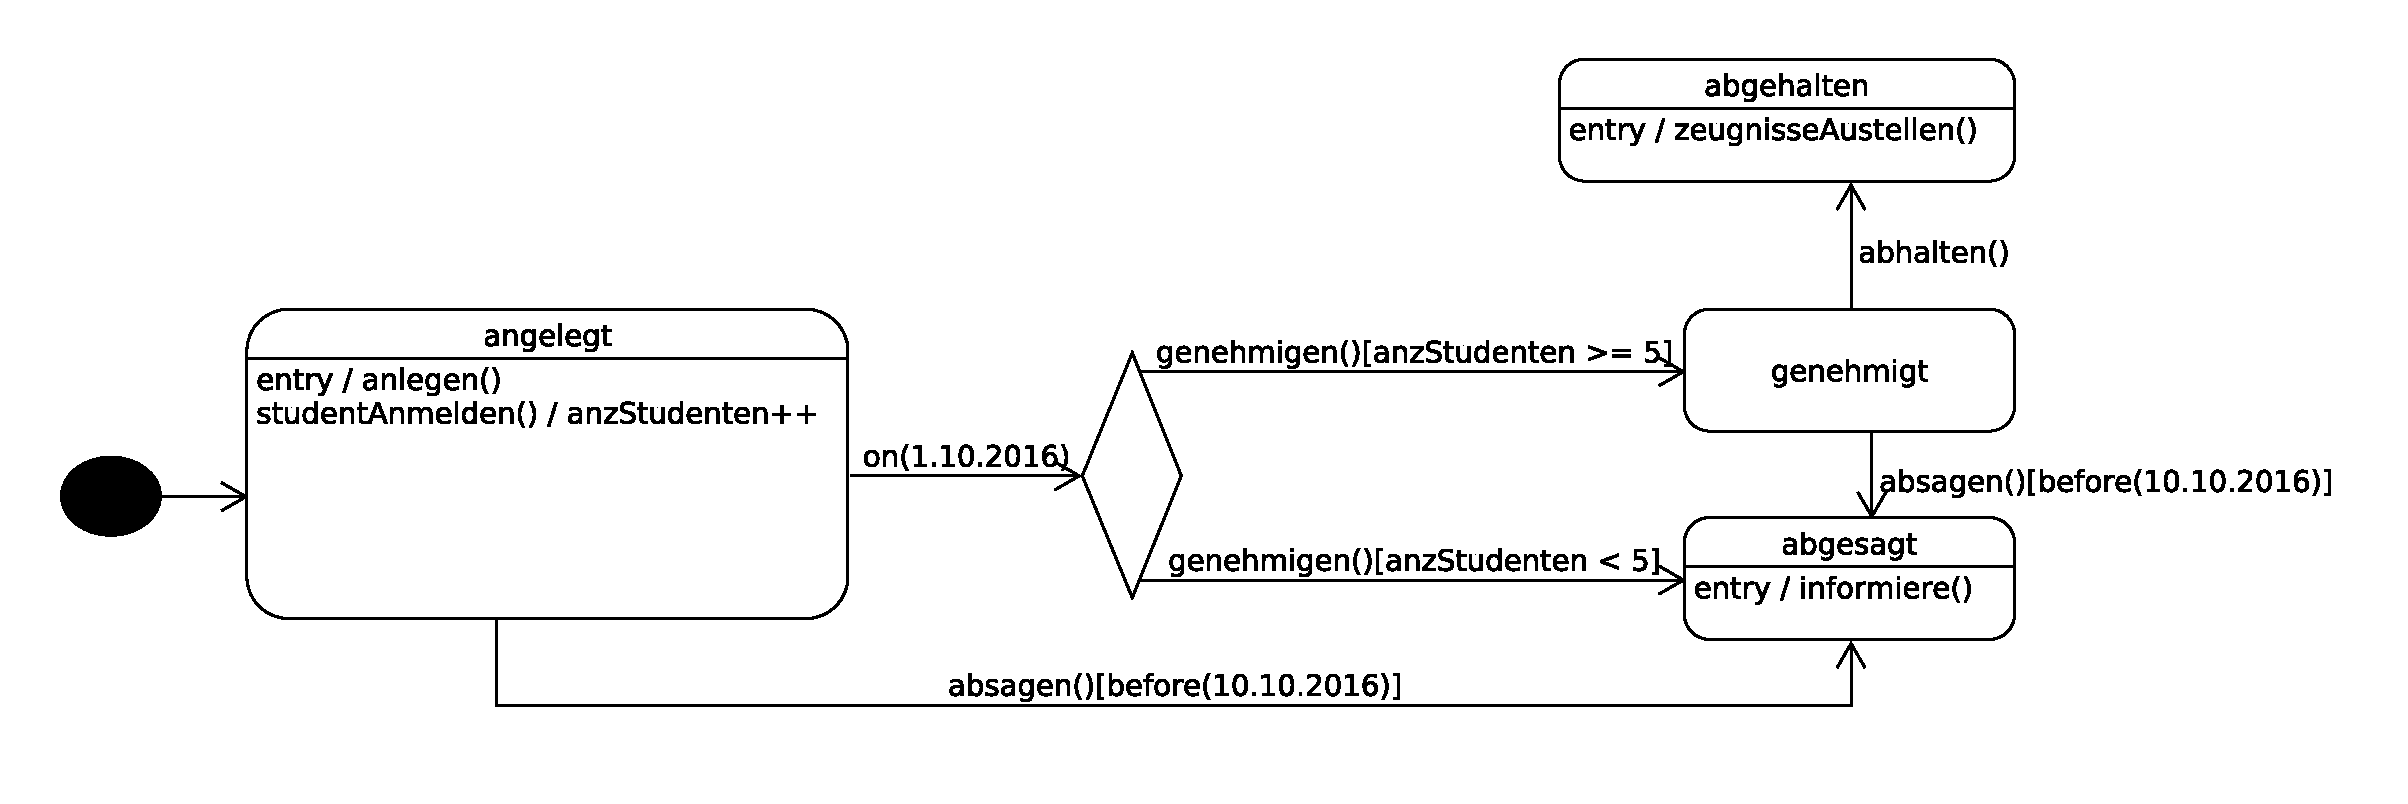
\includegraphics[scale=0.4]{Aufgabe4.eps}
    \end{center}
    
  \end{solution}


\end{document}